%% LyX 2.3.2 created this file.  For more info, see http://www.lyx.org/.
%% Do not edit unless you really know what you are doing.
\documentclass[english,aspectratio=169,handout]{beamer}
\usepackage{mathptmx}
\usepackage{eulervm}
\usepackage[T1]{fontenc}
\usepackage[latin9]{inputenc}
\usepackage{babel}
\usepackage{amsmath}
\usepackage{amssymb}
\usepackage{dsfont}
\ifx\hypersetup\undefined
  \AtBeginDocument{%
    \hypersetup{unicode=true,pdfusetitle,
 bookmarks=true,bookmarksnumbered=false,bookmarksopen=false,
 breaklinks=false,pdfborder={0 0 0},pdfborderstyle={},backref=false,colorlinks=true,
 allcolors=NYUPurple,urlcolor=LightPurple}
  }
\else
  \hypersetup{unicode=true,pdfusetitle,
 bookmarks=true,bookmarksnumbered=false,bookmarksopen=false,
 breaklinks=false,pdfborder={0 0 0},pdfborderstyle={},backref=false,colorlinks=true,
 allcolors=NYUPurple,urlcolor=LightPurple}
\fi

\makeatletter

%%%%%%%%%%%%%%%%%%%%%%%%%%%%%% LyX specific LaTeX commands.
%% Because html converters don't know tabularnewline
\providecommand{\tabularnewline}{\\}

%%%%%%%%%%%%%%%%%%%%%%%%%%%%%% Textclass specific LaTeX commands.
% this default might be overridden by plain title style
\newcommand\makebeamertitle{\frame{\maketitle}}%
% (ERT) argument for the TOC
\AtBeginDocument{%
  \let\origtableofcontents=\tableofcontents
  \def\tableofcontents{\@ifnextchar[{\origtableofcontents}{\gobbletableofcontents}}
  \def\gobbletableofcontents#1{\origtableofcontents}
}

%%%%%%%%%%%%%%%%%%%%%%%%%%%%%% User specified LaTeX commands.
\usetheme{CambridgeUS} 
\beamertemplatenavigationsymbolsempty


% Set Color ==============================
\definecolor{NYUPurple}{RGB}{87,6,140}
\definecolor{LightPurple}{RGB}{165,11,255}


\setbeamercolor{title}{fg=NYUPurple}
%\setbeamercolor{frametitle}{fg=NYUPurple}
\setbeamercolor{frametitle}{fg=NYUPurple}

\setbeamercolor{background canvas}{fg=NYUPurple, bg=white}
\setbeamercolor{background}{fg=black, bg=NYUPurple}

\setbeamercolor{palette primary}{fg=black, bg=gray!30!white}
\setbeamercolor{palette secondary}{fg=black, bg=gray!20!white}
\setbeamercolor{palette tertiary}{fg=gray!20!white, bg=NYUPurple}

\setbeamertemplate{headline}{}

\setbeamercolor{parttitle}{fg=NYUPurple}
\setbeamercolor{sectiontitle}{fg=NYUPurple}
\setbeamercolor{sectionname}{fg=NYUPurple}
\setbeamercolor{section page}{fg=NYUPurple}

\AtBeginSection[]{
  \begin{frame}
  \vfill
  \centering
\setbeamercolor{section title}{fg=NYUPurple}
 \begin{beamercolorbox}[sep=8pt,center,shadow=true,rounded=true]{title}
    \usebeamerfont{title}\usebeamercolor[fg]{title}\insertsectionhead\par%
  \end{beamercolorbox}
  \vfill
  \end{frame}
}

\makeatother

\begin{document}
\global\long\def\reals{\mathbf{R}}%
 
\global\long\def\integers{\mathbf{Z}}%
 
\global\long\def\naturals{\mathbf{N}}%
 
\global\long\def\rationals{\mathbf{Q}}%
 
\global\long\def\ca{\mathcal{A}}%
 
\global\long\def\cb{\mathcal{B}}%
 
\global\long\def\cc{\mathcal{C}}%
 
\global\long\def\cd{\mathcal{D}}%
 
\global\long\def\ce{\mathcal{E}}%
 
\global\long\def\cf{\mathcal{F}}%
 
\global\long\def\cg{\mathcal{G}}%
 
\global\long\def\ch{\mathcal{H}}%
 
\global\long\def\ci{\mathcal{I}}%
 
\global\long\def\cj{\mathcal{J}}%
 
\global\long\def\ck{\mathcal{K}}%
 
\global\long\def\cl{\mathcal{L}}%
 
\global\long\def\cm{\mathcal{M}}%
 
\global\long\def\cn{\mathcal{N}}%
 
\global\long\def\co{\mathcal{O}}%
 
\global\long\def\cp{\mathcal{P}}%
 
\global\long\def\cq{\mathcal{Q}}%
 
\global\long\def\calr{\mathcal{R}}%
 
\global\long\def\cs{\mathcal{S}}%
 
\global\long\def\ct{\mathcal{T}}%
 
\global\long\def\cu{\mathcal{U}}%
 
\global\long\def\cv{\mathcal{V}}%
 
\global\long\def\cw{\mathcal{W}}%
 
\global\long\def\cx{\mathcal{X}}%
 
\global\long\def\cy{\mathcal{Y}}%
 
\global\long\def\cz{\mathcal{Z}}%
 
\global\long\def\ind#1{1(#1)}%
 %\newcommand{\pr}{P}
\global\long\def\pr{\mathbb{P}}%
 
\global\long\def\predsp{\cy}%
 %{\hat{\cy}}
\global\long\def\outsp{\cy}%

\global\long\def\prxy{P_{\cx\times\cy}}%
 
\global\long\def\prx{P_{\cx}}%
 
\global\long\def\prygivenx{P_{\cy\mid\cx}}%
 %\newcommand{\ex}{E}
\global\long\def\ex{\mathbb{E}}%
 
\global\long\def\var{\textrm{Var}}%
 
\global\long\def\cov{\textrm{Cov}}%
 
\global\long\def\sgn{\textrm{sgn}}%
 
\global\long\def\sign{\textrm{sign}}%
 
\global\long\def\kl{\textrm{KL}}%
 
\global\long\def\law{\mathcal{L}}%
 
\global\long\def\eps{\varepsilon}%
 
\global\long\def\as{\textrm{ a.s.}}%
 
\global\long\def\io{\textrm{ i.o.}}%
 
\global\long\def\ev{\textrm{ ev.}}%
 
\global\long\def\convd{\stackrel{d}{\to}}%
 
\global\long\def\eqd{\stackrel{d}{=}}%
 
\global\long\def\del{\nabla}%
 
\global\long\def\loss{\ell}%
 
\global\long\def\risk{R}%
 
\global\long\def\emprisk{\hat{R}}%
 
\global\long\def\lossfnl{L}%
 
\global\long\def\emplossfnl{\hat{L}}%
 
\global\long\def\empminimizer#1{\hat{#1}^{*}}%
 
\global\long\def\minimizer#1{#1^{*}}%
\global\long\def\optimizer#1{#1^{*}}%
 
\global\long\def\etal{\textrm{et. al.}}%
 
\global\long\def\tr{\operatorname{tr}}%

\global\long\def\trace{\operatorname{trace}}%
 
\global\long\def\diag{\text{diag}}%
 
\global\long\def\rank{\text{rank}}%
 
\global\long\def\linspan{\text{span}}%
 
\global\long\def\spn{\text{span}}%
 
\global\long\def\proj{\text{Proj}}%
 
\global\long\def\argmax{\operatornamewithlimits{arg\, max}}%
 
\global\long\def\argmin{\operatornamewithlimits{arg\, min}}%

\global\long\def\bfx{\mathbf{x}}%
 
\global\long\def\bfy{\mathbf{y}}%
 
\global\long\def\bfl{\mathbf{\lambda}}%
 
\global\long\def\bfm{\mathbf{\mu}}%
 
\global\long\def\calL{\mathcal{L}}%

\global\long\def\vw{\boldsymbol{w}}%
 
\global\long\def\vx{\boldsymbol{x}}%
 
\global\long\def\vxi{\boldsymbol{\xi}}%
 
\global\long\def\valpha{\boldsymbol{\alpha}}%
 
\global\long\def\vbeta{\boldsymbol{\beta}}%
 
\global\long\def\vsigma{\boldsymbol{\sigma}}%
\global\long\def\vtheta{\boldsymbol{\theta}}%
 
\global\long\def\vd{\boldsymbol{d}}%
 
\global\long\def\vs{\boldsymbol{s}}%
 
\global\long\def\vt{\boldsymbol{t}}%
 
\global\long\def\vh{\boldsymbol{h}}%
 
\global\long\def\ve{\boldsymbol{e}}%
 
\global\long\def\vf{\boldsymbol{f}}%
 
\global\long\def\vg{\boldsymbol{g}}%
 
\global\long\def\vz{\boldsymbol{z}}%
 
\global\long\def\vk{\boldsymbol{k}}%
 
\global\long\def\va{\boldsymbol{a}}%
 
\global\long\def\vb{\boldsymbol{b}}%
 
\global\long\def\vv{\boldsymbol{v}}%
 
\global\long\def\vy{\boldsymbol{y}}%

\global\long\def\dom{\textrm{\textbf{dom} }}%
\global\long\def\rank{\text{\textbf{rank }}}%
\global\long\def\conv{\textrm{\textbf{conv} }}%
\global\long\def\relint{\text{\textbf{relint }}}%
\global\long\def\aff{\text{\textbf{aff }}}%

\global\long\def\hil{\ch}%
 
\global\long\def\rkhs{\hil}%
 
\global\long\def\ber{\text{Ber}}%

\title[DS-GA 1003 / CSCI-GA 2567]{Bootstrap, Bagging, Random Forest and Adaboost Questions\\}
\author{Xintian Han}
\date{}
\institute{CDS, NYU}

\makebeamertitle
\mode<article>{Just in article version}

%\begin{frame}{Contents}
%
%\tableofcontents{}
%\end{frame}
\begin{frame}{Question 1: What is random?}
Which of the followings are random?
\begin{itemize}
\item statistic
\item parameter
\item point estimator
\item sampling distribution
\item standard error
\item bias and variance of a point estimator
\item bootstrap sample
\end{itemize}
 \end{frame}
%
\begin{frame}{[Solution] Question 1: What is random?}
Which of the followings are random?
\begin{itemize}
\item statistic is any function of the data. It is random since we're considering the data is random.
\pause{}
\item parameter is any function of the distribution. It is not random.
\item point estimator is some statistic which is to serve as a ``best guess'' of an unknown parameter. It is random.
\item sampling distribution is not random
\item standard error is a parameter of the sampling distribution. It is not random.
\item bias and variance of a point estimator are still parameters of the sampling distribution of the point estimator. It is not random.
\item bootstrap sample are random samples from the data. It is random.
\end{itemize}
 \end{frame}
%
\begin{frame}{Question 2: Bias and Variance}
Suppose we have samples $X_1,\dots, X_N$ from Normal$(\mu,\sigma^2	)$.
\begin{itemize}
\item What is the maximum likelihood estimator $\hat\mu, \hat\sigma^2$ of the parameter $\mu$, $\sigma^2$?
\item Are the maximum likelihood estimator unbiased? If not, how do we fix it?
\item What is the sampling distribution of $\hat\mu$? What is the variance of the estimator $\hat\mu$?
\end{itemize}

\end{frame}
%
\begin{frame}{[Solution] Question 2: Bias and Variance}
Suppose we have samples $X_1,\dots, X_N$ from Normal$(\mu,\sigma^2	)$.
\begin{itemize}
\item What is the maximum likelihood estimator $\hat\mu, \hat\sigma^2$ of the parameter $\mu$, $\sigma^2$?
\begin{align*}
\hat\mu = 	\bar{X} = \frac{1}{N}\sum_{i=1}^N X_i; \quad \hat{\sigma}^2&= \frac{1}{N}\sum_{i=1}^N(X_i-\bar{X})^2
\end{align*}
\pause{}
\item Are the maximum likelihood estimator unbiased? If not, how do we fix it?
\[
\mathbb{E} \hat\mu = \mu; \quad \mathbb{E} \hat{\sigma}^2 = \frac{N-1}{N}\sigma^2
\]
So $\hat {\mu}$ is unbiased but $\hat{\sigma}^2$ is not unbiased. $\frac{1}{N-1}\sum_{i=1}^N(X_i-\bar{X})^2
$ is an unbiased estimator of $\sigma^2$.
\pause{} 
\item What is the sampling distribution of $\hat\mu$? What is the variance of the estimator $\hat\mu$?

Sampling distribution is Normal $(\mu, \sigma^2/N)$. Variance of the estimator is $\sigma^2/N$.
\end{itemize}

\end{frame}
%
\begin{frame}{Question 3: Bootstrap}
Let $X_1,\dots,X_{2n+1}$ be an i.i.d.~sample from a distribution.
  To estimate the median of the distribution, you can compute the sample
  median of the data.
  \begin{enumerate}
  \item How do we compute an estimate of the variance of
    the sample median?
  \item How do we compute an estimate of a 95\% confidence
    interval for the median.
  \end{enumerate}
\end{frame}
%
\begin{frame}{Question 3: Bootstrap}
Let $X_1,\dots,X_{2n+1}$ be an i.i.d.~sample from a distribution.
  To estimate the median of the distribution, you can compute the sample
  median of the data.
  \begin{enumerate}
  \item How do we compute an estimate of the variance of
    the sample median?
\begin{enumerate}
    \item Draw $B$ bootstrap samples $D^{1},\ldots,D^B$ each of size
      $2n+1$.  The samples are formed by drawing uniformly with replacement from
      the original data set $X_1,\ldots,X_{2n+1}$.
      We will make a total of $B(2n+1)$ draws.
    \item For each $D^{i}$ compute the corresponding median $\hat{m}_i$.
    \item Compute the sample variance of the $B$ medians $m_1,\ldots,m_B$.
    \end{enumerate}    
    \pause{}
  \item How do we compute an estimate of a 95\% confidence
    interval for the median. 
        \begin{enumerate}
    \item Draw $B$ bootstrap samples $D^{1},\ldots,D^B$ each of size
      $2n+1$.  The samples are formed by drawing uniformly with replacement from
      the original data set $X_1,\ldots,X_{2n+1}$.
      We will make a total of $B(2n+1)$ draws.
    \item For each $D^{i}$ compute the corresponding median $\hat{m}_i$.
    \item Compute the $2.5\%$ and $97.5\%$ sample quantiles of the
      list $\hat{m}_1,\ldots,\hat{m}_B$.
      Use these as the estimates of the left and right endpoints of
      the confidence interval, respectively.
    \end{enumerate}
  \end{enumerate}
\end{frame}
%
\begin{frame}{[Solution] Question 4: Bagging and Random Forest}
\begin{itemize}
\item 	A slide titled ``Averaging Independent Prediction Functions'' (there are multiple) states that $\mathrm{Var} (\hat{f}_{avg}(x)) = \frac{1}{B^2} \mathrm{Var} \left( \sum_{b=1}^B \hat{f}_b(x)\right) = \frac{1}{B} \mathrm{Var} \left(  \hat{f}_1(x)\right)$. Justify each of the two equality signs. 
\pause{}
\item The above equality gives some intuition as to why bagging might reduce variance. But really, but situation is more complicated: the bootstrap samples used for bagging are not independent. Why not? 
\item If the variance of the individual predictors that we are bagging is $\sigma^2$, and the correlation between them is $\rho^2$, what is the variance of the bagged predictor? 
\item Bagging decision trees leads us to the highly popular random forests. However, to make bagging for decision trees work well, we need one more key idea. What is it?
\end{itemize}
	
\end{frame}
%
\begin{frame}{[Solution] Question 4: Bagging and Random Forest}
\begin{itemize}
\item 	A slide titled ``Averaging Independent Prediction Functions'' (there are multiple) states that $\mathrm{Var} (\hat{f}_{avg}(x)) = \frac{1}{B^2} \mathrm{Var} \left( \sum_{b=1}^B \hat{f}_b(x)\right) = \frac{1}{B} \mathrm{Var} \left(  \hat{f}_1(x)\right)$. Justify each of the two equality signs. 

$\mathrm{Var} \left(\frac{1}{B} \sum_{b=1}^B \hat{f}_b(x)\right) $. $\hat{f}_1(x), \hat{f}_2(x), \dots, \hat{f}_B(x)=\frac{1}{B^2} \mathrm{Var} \left( \sum_{b=1}^B \hat{f}_b(x)\right) 
$ are independent prediction functions. So \[\frac{1}{B^2} \mathrm{Var} \left( \sum_{b=1}^B \hat{f}_b(x)\right) = \frac{1}{B^2} B*\mathrm{Var} \left(  \hat{f}_1(x)\right) = \frac{1}{B} \mathrm{Var} \left(  \hat{f}_1(x)\right)\]
\pause{}
\item The above equality gives some intuition as to why bagging might reduce variance. But really, but situation is more complicated: the bootstrap samples used for bagging are not independent. Why not? 

A bootstrap sample from $\cd_n=(x_1,\dots,x_n)$ is a sample of size $n$ drawn with replacement from $\cd_n$. So there can be overlaps between bootstrap samples.
\end{itemize}
\end{frame}
\begin{frame}{[Solution] Question 4: Bagging and Random Forest}
\begin{itemize}
\item If the variance of the individual predictors that we are bagging is $\sigma^2$, and the correlation between them is $\rho^2$, what is the variance of the bagged predictor? 
\[\text{Var}(\frac{1}{B}\sum_{b=1}^B\hat{f}_b) = \frac{1}{B^2}*(B*\text{Var}(\hat f_1(x))+B(B-1)*\text{Cov}(\hat f_1(x),\hat f_2(x)))=\frac{1}{B}\sigma^2+\frac{B-1}{B}\rho^2\]
\pause{}
\item Bagging decision trees leads us to the highly popular random forests. However, to make bagging for decision trees work well, we need one more key idea. What is it?

We randomly sample features when building trees to reduce the covariance between trees.
\end{itemize}
	
\end{frame}	
%
\begin{frame}{Question 5: Adaboost-Concept Check\footnote{From MIT exams}}
Decide whether each of the statements below is true or false.
\begin{itemize}
\item If a weak classifier has a weighted error rate $\epsilon \leq 1/3$, it can only misclassify up to $1/3$ of the training points.
\item The error rate of the ensemble classifier never increases from one round to the next.
\item Adaboost accounts for outliers by lowering the weights of training points that are repeatedly misclassified.
\item When you update weights, the training point with the smallest weight in the previous round will always increase in weight.
\end{itemize}	
\end{frame}
%
\begin{frame}{Adaboost Algorithm}
Given training set $\cd=\left\{ \left(x_{1},y_{1}\right),\ldots,\left(x_{n},y_{n}\right)\right\} $.
\begin{enumerate}
\item Initialize observation weights $w_{i}=1$, $i=1,2,\ldots,n$.

\pause{}
\item For $m=1$ to $M$:
\begin{enumerate}
\item Base learner fits weighted training data and returns $G_{m}(x)$

\pause{}
\item Compute \textbf{weighted empirical 0-1 risk}:
\[
\mbox{err}_{m}=\frac{1}{W}\sum_{i=1}^{n}w_{i}\ind{y_{i}\neq G_{m}(x_{i})}\quad\text{where }W=\sum_{i=1}^{n}w_{i}.
\]


\pause{}
\item Compute $\alpha_{m}=\ln\left(\frac{1-\text{err}_{m}}{\text{err}_{m}}\right)$
{[}\textbf{classifier weight}{]}

\pause{}
\item Set $w_{i}\gets w_{i}\cdot\exp\left[\alpha_{m}\ind{y_{i}\neq G_{m}(x_{i})}\right],\quad i=1,2,\ldots,n$
{[}\textbf{example weight adjustment}{]}

\pause{}
\end{enumerate}
\item Ouptut $G(x)=\sign\left[\sum_{m=1}^{M}\alpha_{m}G_{m}(x)\right]$.
\end{enumerate}	
\end{frame}
%
\begin{frame}{Question 5: Adaboost-Concept}
Decide whether each of the statements below is true or false.
\begin{itemize}
\item If a weak classifier has a weighted error rate $\epsilon \leq 1/3$, it can only misclassify up to $1/3$ of the training points.

\textbf{False}. We use weighted error rate.
\pause{}
\item The error rate of the ensemble classifier never increases from one round to the next.

\textbf{False}. There is no guarantee for error rate not to increase from one round to the next.
\pause{}
\item Adaboost accounts for outliers by lowering the weights of training points that are repeatedly misclassified.

\textbf{False}. Adaboost will increase the weights of training points that are repeatedly misclassified.
\pause{}
\item When you update weights, the training point with the smallest weight in the previous round will always increase in weight.

\textbf{False}. It will increase weight only if it is misclassified in the current round. 
\pause{}
\end{itemize}	
\end{frame}
%
\begin{frame}{Question 6: Adaboost-Algorithm\footnote{From CMU exams}}
Consider building an ensemble of decision stumps Gm with the AdaBoost algorithm,
\[
f(x) = \text{sign} \left( \sum_{m=1}^M\alpha_m G_m (x)\right)
\]
Figure displays a few labeled point in two dimensions as well as the first stump we have chosen. A stump predicts binary $\pm 1$ values, and depends only on one coordinate value (the split point). The little arrow in the figure is the normal to the stump decision boundary indicating the positive side where the
stump predicts $+1$. All the points start with uniform weights.
\begin{itemize}
\item Circle all the point(s) in Figure 1 whose weight will increase as a result of incorporating the
first stump (the weight update due to the first stump).
\item Draw in the same figure a possible stump that we could select at the next boosting iteration.
You need to draw both the decision boundary and its positive orientation.

\item Will the second stump receive higher coefficient in the ensemble than the first? In other
words, will 
$\alpha_2 > \alpha_1$? Briefly explain your answer. (no calculation should be necessary).	
\end{itemize}

\end{frame}
%
\begin{frame}{Question 6:Adaboost-Algorithm}
\begin{center}
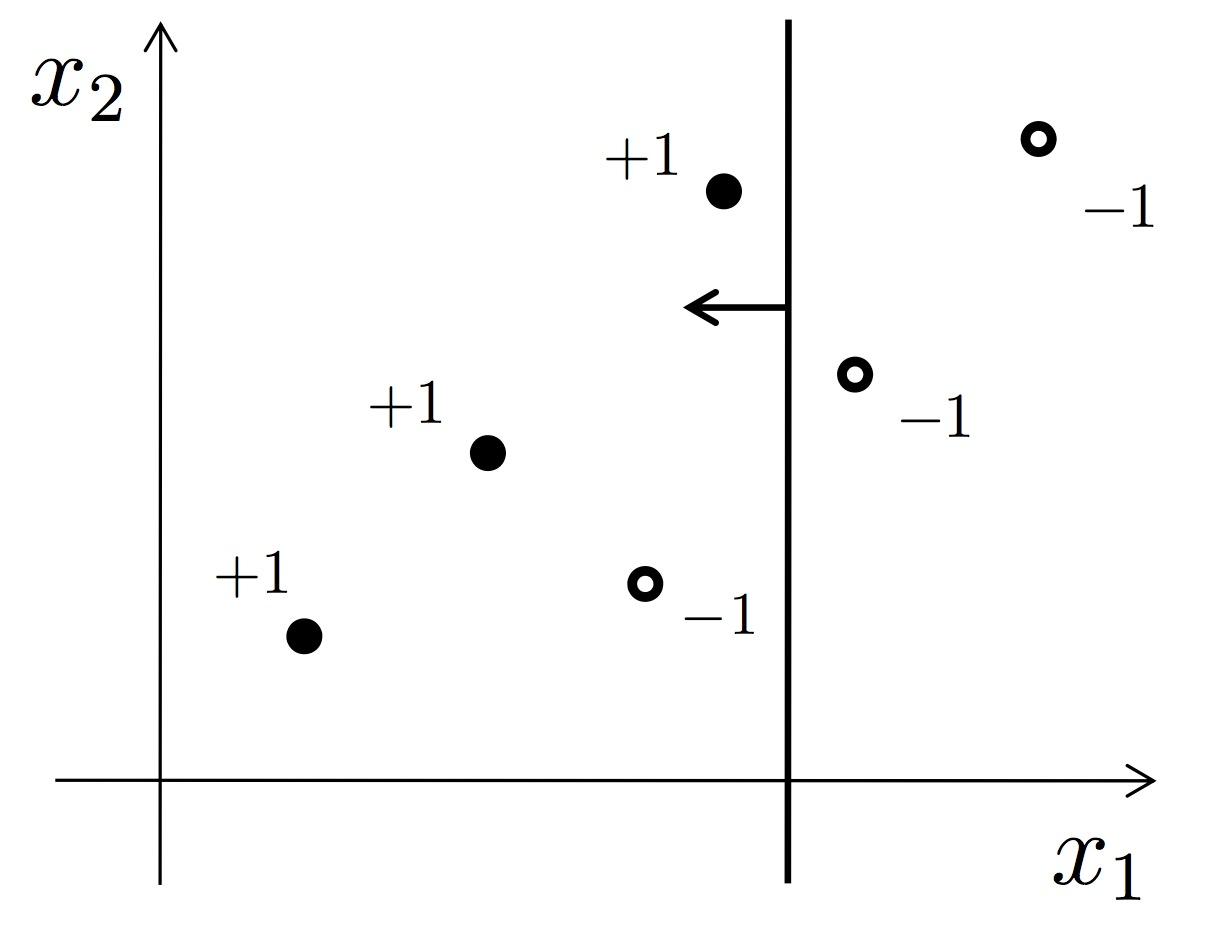
\includegraphics[width = 8cm]{../Figures/Boosting/Adaboost_question}	
\end{center}
\end{frame}
%
\begin{frame}{Question 6:Adaboost-Algorithm}
\begin{itemize}
\item Circle all the point(s) in Figure 1 whose weight will increase as a result of incorporating the
first stump (the weight update due to the first stump).

(sol.) The only misclassified negative sample.
\item Draw in the same figure a possible stump that we could select at the next boosting iteration.
You need to draw both the decision boundary and its positive orientation.

(sol.) The second stump will also be a vertical split between the second positive sample (from left
to right) and the misclassified negative sample, as drawn in the figure.
\item Will the second stump receive higher coefficient in the ensemble than the first? In other
words, will 
$\alpha_2 > \alpha_1$? Briefly explain your answer. (no calculation should be necessary).	

(sol.) $\alpha_2 > \alpha_1$ because the point that the second stump misclassifies will have a smaller relative
weight since it is classified correctly by the first stump.
\end{itemize}

\end{frame}
\end{document}
